\documentclass{article}
\usepackage[utf8]{inputenc}
\usepackage[francais]{babel}
\usepackage[T1]{fontenc}

\usepackage[hmarginratio=1:1,top=32mm,columnsep=15pt]{geometry}
\usepackage{multicol}
\geometry{margin=1.6cm}

\usepackage{amssymb}
\setcounter{tocdepth}{3}
\usepackage{graphicx}

\usepackage{fancyhdr}

\pagestyle{fancy}
\fancyhf{}
\rhead{LO17 - Rapport de projet Indexation et recherche d'information}
\lhead{Théophile DANCOISNE et Samuel Reymondet}
\rfoot{Page \thepage}

\usepackage{listings}
\usepackage{color}
 
\definecolor{codegreen}{rgb}{0,0.6,0}
\definecolor{codegray}{rgb}{0.5,0.5,0.5}
\definecolor{codepurple}{rgb}{0.58,0,0.82}
\definecolor{backcolour}{rgb}{0.95,0.95,0.92}
 
\lstdefinestyle{mystyle}{
    backgroundcolor=\color{backcolour},   
    commentstyle=\color{codegreen},
    keywordstyle=\color{magenta},
    numberstyle=\tiny\color{codegray},
    stringstyle=\color{codepurple},
    basicstyle=\footnotesize,
    breakatwhitespace=false,         
    breaklines=true,                 
    captionpos=b,                    
    keepspaces=true,                 
    numbers=left,                    
    numbersep=5pt,                  
    showspaces=false,                
    showstringspaces=false,
    showtabs=false,                  
    tabsize=4
}
 
\lstset{style=mystyle}

\title{LO17 - Rapport de projet - Indexation et recherche d'information}
\author{Théophile DANCOISNE et Samuel Reymondet}
\date{Automne 2017}

\begin{document}

\maketitle

% TODO: blabla d'introduction sur les objectifs; petite note sur les technos utilisées

\section{Préparation du Corpus}
%TODO: blabla d'intro

\subsection{Découverte et exploration du la structure des données}
Avant même de prendre connaissance des différents éléments à extraire, nous avons exploré à l'aveugle les différents fichiers html à notre disposition. Avec un fichier html, on disposede la source du contenu et de sa mise en forme, et l'on peut facilement l'affichier de manière formattée via un navigateur. Ainsi, nous avons ouvert plusieurs pages, en comparant l'affichage et la manière donc le code html est structuré. L'outil principal utilisé ici est l'inspecteur de source intégré au navigateur. Ce dernier permet notamment de naviguer visuellement parmi les différents éléments de la page à travers le code source. Pour nos besoins, cet outil permet ainsi d'identifier des schémas permettant d'accéder aux éléments d'importance. Dès le départ, nous avons repéré que les classes CSS des différents éléments d'écrivant les articles permettent de les identifier de manière quasiment unique. C'est cette méthode que nous avons utilisée.

\subsection{Méthode d'extraction des données}
Après avoir pris connaissance des éléments à extraire dont le numéro du bulletin, la date, la rubirque, etc., nous avons pu établir une stratégie de captation de ces éléments. Comme pour la majorité des extractions depuis des fichiers xml, nous avons utilisé le très simple XPath (XML Path Language), un outil de requête de sélection de nodes dans un document html. A l'aide d'XPath, il est ainsi possible de seléction des éléments de manière rigoureuse à travers une syntaxe condensée mais intuitive.
L'identification de la relation de quasi-unicité entre les classes des éléments et de leur type nous a grandement facilité la tâche. En effet, il nous a suffit d'identifié la classe de chaque élément d'important pour pouvoir y accéder très simplement. Par exemple le titre porte la classe "style17". La requête XPath correspondante est donc:
\begin{lstlisting}
//*[@class="style17"]
\end{lstlisting}
La seule subtilité lors de cette partie a été pour le contenu de l'article de concaténer tous les paragraphes retournés par la requête:
\begin{lstlisting}
//*[@width="452"]//*[@class="style95"]
\end{lstlisting}

\subsection{Vérifications de la qualité de l'extraction}
% TODO: décrire la méthode utilisée pour les images (compter de 2 manières différentes) et pour le contenu des articles (pour 15 articles aléatoire afficher la première et la dernière ligne de l'article. Et aussi vérification à la main.

\section{Indexation du Corpus}
% TODO: préciser la petite erreur sémantique introduite en utilisant le terme de bulletin au lieu d'article

\subsection{Création d'une stop-list}
% TODO: présenter les 3 fichiers, dire que l'on a exploité les mots des titres et des contenus.

% TODO: parler de la manière dont on interprète un "mot" (entouré d'espace, sans quote, juste les caractères alphanumériques...) => impacte sur les résultats.

Méthode subjective
\begin{figure}
\begin{center}
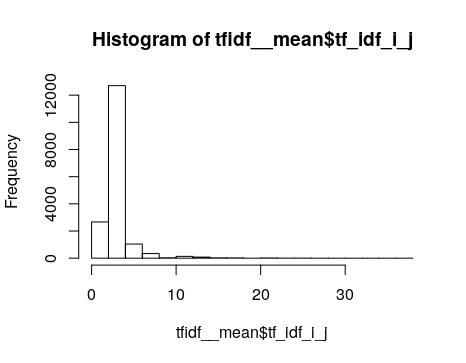
\includegraphics{rapport/hist_tfidf.png}
\end{center}
\end{figure}

Méthode objective
\begin{figure}
\begin{center}
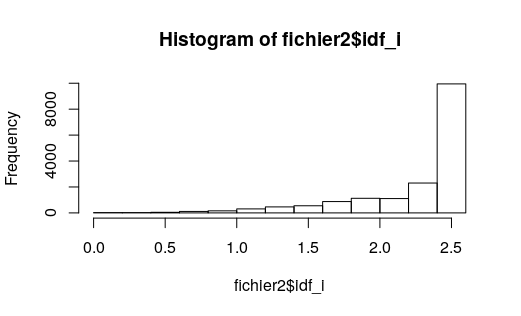
\includegraphics{rapport/hist_idf.png} 
\end{center}
\end{figure}

3ème quartile (trouver le mot correspondant)
Moyenne 2.226, médianne 2.513 et 3ème quartile 2.513. => Sélection de la médiane.
% TODO: décrire en détails notre analyse

Une fois que notre stop-list a été créée nous avons pu recréer un fichier XML ne contenant que les termes significatifs selon notre critère.

\subsection{Création des lemmes}
% TODO: décrire les pipes effectués

\subsection{Création des fichiers inverses}
% TODO: décrire les pipes effectués

\section{Correcteur orthographique}
Au sein de cette itération, nous avons mis en place un correcteur ortographique en associant un lemme à chaque mot d'une phrase saisie. Pour cela nous avons créé une classe Lexique qui charge un lexique de lemmes lors de son instanciation. La structure de données utilisée pour le lexique en tant que tel est un table de hashing associant à chaque mot son lemme, avec une recherche en $O(n)$, avec $n$ le nombre de mots dans la table.

Comme précedemment, nous avons réimplémenté des scripts en Python mais en conservant une architecture souple orientée objet. Autrement dit les concepts sont les mêmes mais dans un langage différent.

Si un mot n'est pas disponible dans le lexique, alors le lemme du mot le plus suffisamment ressemblant est retourné. Pour quantifier cette "ressemblance", nous avons mis en place un algorithme de proximité et un algorithme de calcul de distance de Levenshtein. Ces deux algorithmes ont été implémentées au sein de la classe en tant que méthodes.

L'algorithme de proximité est très simple. Pour deux mots dont on souhaite calculer la proximité, on accorde un point par lettre identique à la même position dans les mots. Nous ne considérons que les proximités des mots du lexique supérieurs à 3 lettres, limite fixée en attribut de la classe.

% TODO: description distance de Levenshtein

\end{document}
